\chapter{実験}
\label{chap:ex}

%----------------------------------------------
\section{まえがき}
%----------------------------------------------
前章で提案したDNNに基づくパーミュテーション解決法の有効性を確認するために,FDICAで分離した信号を模倣した行列を用意し,提案パーミュテーション解決法を適用した後に,その性能を評価した.
\ref{sec:ex_condition}節では,本実験における条件を詳細に示し,\ref{sec:ex_res}節では提案手法のパーミュテーション解決性能を示している.
\ref{sec:matome}節で本章のまとめを述べる.
%----------------------------------------------
\section{実験条件}
\label{sec:ex_condition}
%----------------------------------------------
% \begin{table}[t]
% \begin{center}
%  \caption{Experimental conditions}
%  \label{table:ex}
%   \begin{tabular}{clll}\hline \hline
%    Window function in STFT & Hamming window  \\ \hline
%    Window length in STFT & 512~ms  \\ \hline
%    Shift length in STFT & 128~ms \\ \hline
%    Paramaters in Adam optimizer & \begin{tabular}{c}
%    \begin{flushleft}Learning rate = $0.001$\end{flushleft}\\
%    \begin{flushleft}$\beta = 0.9$\end{flushleft}
%    \end{tabular}  \\ \hline 
%    Reverberation time & $T_{60} = 470$~ms\\ \hline
%    Source direction of training data & $(\theta_1, \theta_2)=(60^\circ, 120^\circ)$\\ \hline
%    Source direction of test data & \begin{tabular}{c}
%    \begin{flushleft}(\theta_1, \theta_2)=(60^\circ, 120^\circ)\end{flushleft}\\ 
%    \begin{flushleft}(\theta_1, \theta_2)=(60^\circ, 100^\circ)\end{flushleft}\\ 
%    \begin{flushleft}(\theta_1, \theta_2)=(70^\circ, 110^\circ)\end{flushleft}
%    \end{tabular}\\ \hline \hline
%   \end{tabular}
%  \end{center}
% \end{table}

\begin{table}[t]
\begin{center}
 \caption{Speech sources obtained from SiSEC2011}
 \label{table:wav}
  \begin{tabular}{clll}\hline \hline
   Signal & Language & Data name &Length~[s]  \\ \hline
   Speech & English & dev1\_female4\_src\_1 & 10.0  \\ \hline
   Speech & English & dev1\_female4\_src\_2 &  10.0 \\ \hline
   Speech & Japanese & dev1\_female4\_src\_3 & 10.0  \\ \hline
   Speech & Japanese & dev1\_female4\_src\_4 &  10.0 \\ \hline
   Speech & English & dev1\_male4\_src\_1 & 10.0  \\ \hline
   Speech & English & dev1\_male4\_src\_2 &  10.0 \\ \hline
   Speech & Japanese & dev1\_male4\_src\_3 & 10.0  \\ \hline
   Speech & Japanese & dev1\_male4\_src\_4 &  10.0 \\ \hline
   \hline
  \end{tabular}
 \end{center}
\end{table}
%%%%%%%%%%%%%%%%%%%%%%%%%%%%
\begin{figure}[t]
     \vspace{8pt}
    \begin{center}
        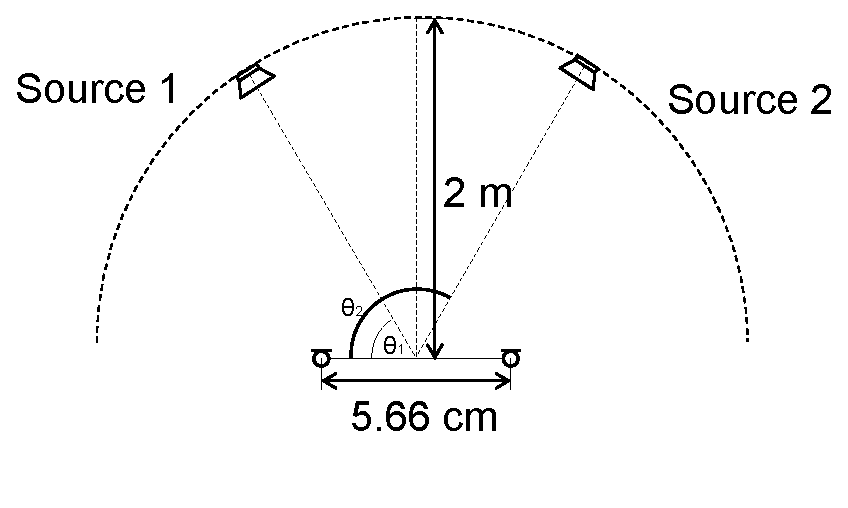
\includegraphics[width=0.8\columnwidth]{figures/mic}
    \end{center}
    \vspace{-8pt}
	\caption{Recording condition of JR2 impulse response.}
	\label{fig:mic}
\end{figure}
%%%%%%%%%%%%%%%%%%%%%%%%%%%%
%%%%%%%%%%%%%%%%%%%%%%%%%%%%
\begin{figure}[t]
    \begin{center}
        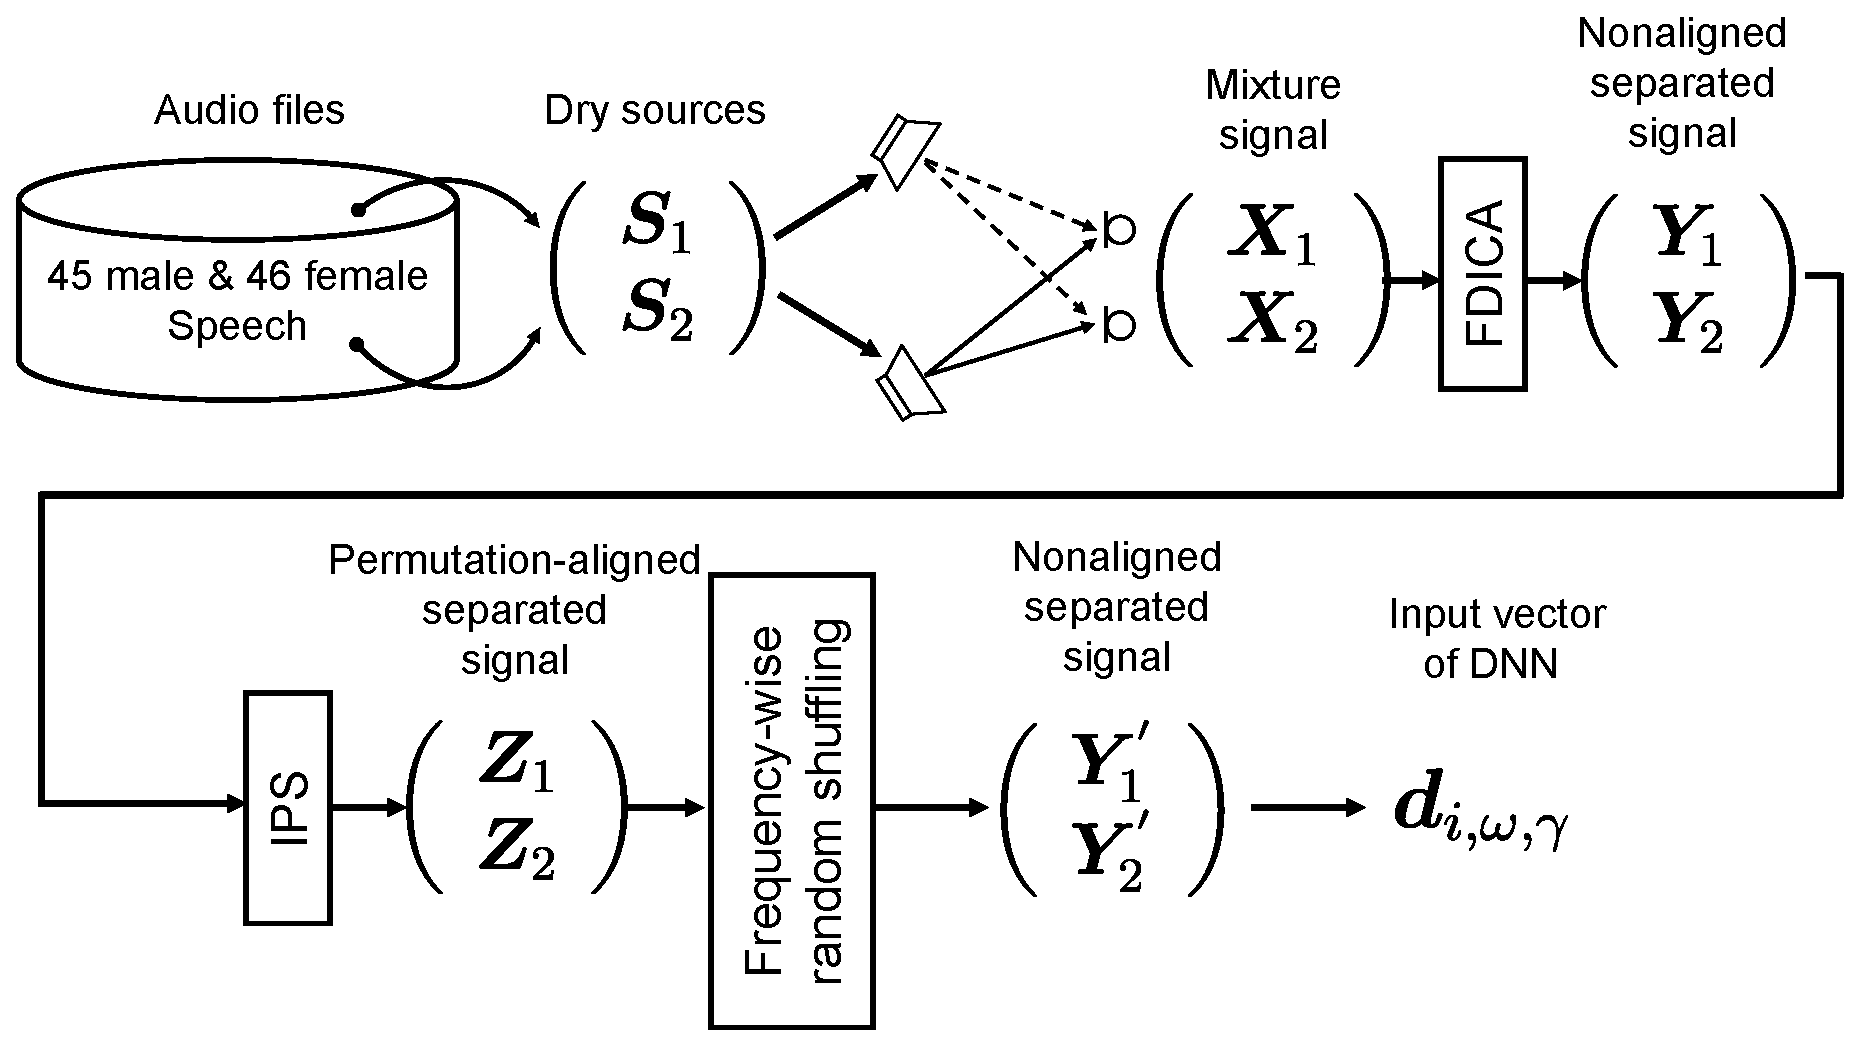
\includegraphics[width=0.999\columnwidth]{figures/make_inputvec.eps}
    \end{center}
    \vspace{-8pt}
	\caption{Process flow of producing input vectors for DNN.}
	\label{fig:make_inputvec}
\end{figure}
%%%%%%%%%%%%%%%%%%%%%%%%%%%%

本実験では,提案するDNNに基づくパーミュテーション解決法において,どの程度各周波数成分の並び替えができるかについて実験的に確認する.
実験データとして,全ての成分が0か1の行列,25列毎に0と1の値が入れ替わる行列,1列毎に0と1の値が入れ替わる行列の3パターンを使用する.
また,FDICAにはブロックパーミュテーションと呼ばれる,ブロック単位で音源分離に失敗することより,2ブロック,4ブロック,8ブロック単位で各周波数をシャッフルした実験も同時に実施した.
学習データには,完全分離信号$\bm{Z}_1$と$\bm{Z}_2$を各周波数ごとにランダムでシャッフルしたものを用いる.
検証データには学習データにはないパターンで$\bm{Z}_1$と$\bm{Z}_2$をシャッフルさせることで作成する.即ち,検証データは実際にはテストデータとも言える.
DNNの最適化法にはAdamを用い,ハイパーパラメータはそれぞれ$\varepsilon=1.0\times10^{-8},~\beta_1 = 0.9,~\beta_2 = 0.999$及び学習率$\eta=0.001$とした.
その他の学習パラメータについては,バッチサイズを8,エポック数を1000,学習に用いるシャッフルパターンを300として誤差逆伝搬学習を行った.
主観評価として,各周波数成分において正しく並び替えが行える割合,即ち検証データに対する正答率を用いる.


%----------------------------------------------
\section{実験結果}
\label{sec:ex_res}
%----------------------------------------------
%%%%%%%%%%%%%%%%%%%%%%%%%%%%
\begin{figure}[t]
    \begin{center}
        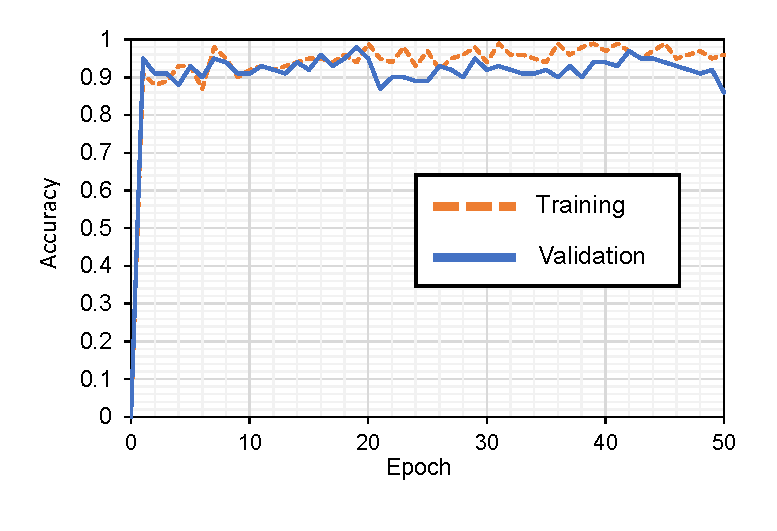
\includegraphics[width=0.85\columnwidth]{figures/accu.eps}
    \end{center}
    \vspace{-8pt}
	\caption{Accuracy curves of DNN for training and validation datasets.}
	\label{fig:accu}
\end{figure}
%%%%%%%%%%%%%%%%%%%%%%%%%%%%

%%%%%%%%%%%%%%%%%%%%%%%%%%%%
\begin{figure}[t]
    \begin{center}
        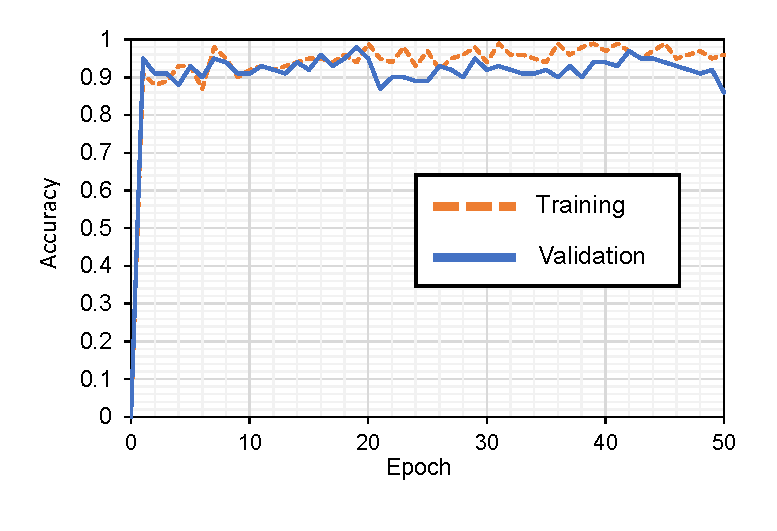
\includegraphics[width=0.85\columnwidth]{figures/accu.eps}
    \end{center}
    \vspace{-8pt}
	\caption{Accuracy curves of DNN for training and validation datasets.}
	\label{fig:01mat}
\end{figure}
%%%%%%%%%%%%%%%%%%%%%%%%%%%%


Fig.~\ref{fig:01mat}〜Fig.~\ref{fig:01_8block}には,01行列の周波数成分に対してそれぞれ1行,2行,4行,8行ごとにシャッフルをランダムに行った時の結果を示す.


%%%%%%%%%%%%%%%%%%%%%%%%%%%%
\begin{figure}[t]
    \begin{center}
        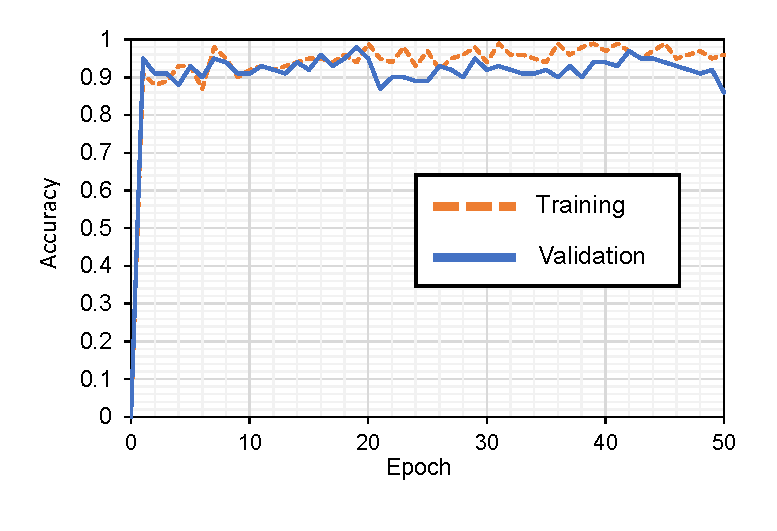
\includegraphics[width=0.85\columnwidth]{figures/accu.eps}
    \end{center}
    \vspace{-8pt}
	\caption{Accuracy curves of DNN for training and validation datasets.}
	\label{fig:25stripe_mat}
\end{figure}
%%%%%%%%%%%%%%%%%%%%%%%%%%%%

Fig.~〜Fig.~には,25列ごとに0と1の値を入れ替えた行列の周波数成分に対してそれぞれ1行,2行,4行,8行ごとにシャッフルをランダムに行った時の結果を示す.
%%%%%%%%%%%%%%%%%%%%%%%%%%%%
\begin{figure}[t]
    \begin{center}
        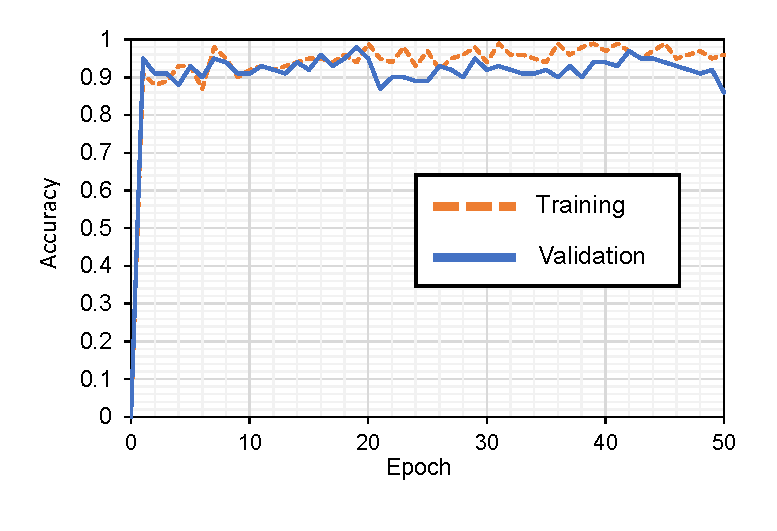
\includegraphics[width=0.85\columnwidth]{figures/accu.eps}
    \end{center}
    \vspace{-8pt}
	\caption{Accuracy curves of DNN for training and validation datasets.}
	\label{fig:stripe_mat}
\end{figure}
%%%%%%%%%%%%%%%%%%%%%%%%%%%%

Fig.~〜Fig.~には,1列ごとに0と1の値を入れ替えた行列の周波数成分に対してそれぞれ1行,2行,4行,8行ごとにシャッフルをランダムに行った時の結果を示す.




Fig.~\ref{fig:accu}に,学習用データ及び検証用データそれぞれのDNN正解率を示す.
この結果から,DNNは周波数毎の正しいパーミュテーションを約85\%の精度で推定できていることが分かる.
つまり,DNNが正しいパーミュテーション推定に失敗する確率は15\%である.
しかし,\ref{sec:maj}節及び\ref{sec:fullband}項で示した通り,時間軸及び周波数軸に沿った多数決を取ることで,これらの予測誤差の悪影響を大幅に軽減することができる.

Figs.~\ref{fig:060-120},\ref{fig:060-100}及び\ref{fig:070-110}に,音源到来方向毎のSDR改善量を示す.
各箱ひげ図は,56個(8個の音声ファイルの全組み合わせ数)の分離実験結果から生成されている.
各箱ひげ図における,四分位範囲(interquartile range: IQR),最大値$b_{max}$及び最小値$b_{min}$は以下のように計算される.
\begin{align}
 \mbox{IQR} &= Q_3 - Q_1 \\
  b_{max} &=   Q_3 +\mbox{IQR} \times 1.5\\
  b_{min} &=   Q_1 -\mbox{IQR} \times 1.5
\end{align}
ここで,$Q_3$及び$Q_1$は,それぞれ第三四分位数及び第一四分位数を示す.
$[b_{min}, b_{max}]$の範囲外の値は,外れ値として扱った.

既に文献~\cite{EU}で報告されているように,どの音源到来方向でもILRMAの分離性能は$4$~dB以下であるのに対し,IPSを用いたFDICAでは約$10$~dB以上の改善を達成している.
この結果から,高残響下にある音声混合信号の分離タスクに対して,ILRMAはしばしば分離に失敗している事がわかる.

提案パーミュテーション解決法を適用したFDICAは,いずれも平均的にILRMAを上回る分離性能を示している.また,提案手法がうまく働いた場合はSDR改善量が$13$~dBに達成するなど,FDICAベースの分離の上限性能に比較的近い性能も確認できた.
しかし,提案DNNの推定間違いの悪影響が,多数決でも軽減できないほど大きな場合は,並び替えに失敗することもある.この場合,$0$~dB以下のSDR改善量となることが多く,この場合はILRMAのブロックパーミュテーションの様に中間の周波数でパーミュテーションが反転していることが考えられる.

Fig.~\ref{fig:DOA}では,音源到来方向の違いによる提案手法のSDR改善量の差を比較している.
\ref{sec:ex_condition}節でも説明したように学習データに使われている音声の到来方向は$(\theta_1, \theta_2)=(60^\circ, 120^\circ)$のみであり,$(\theta_1, \theta_2)=(60^\circ, 100^\circ)$及び$(\theta_1, \theta_2)=(70^\circ, 110^\circ)$の到来方向は,学習データに含まれていない.
しかし,Fig.~\ref{fig:DOA}から分かるように,学習データに存在しない音源到来方法であっても,パーミュテーション解決性能には大きな差が無い.
この結果は,提案DNNが空間情報を学習しているのではなく,文献~\cite{COR}のように,ある種の類似度を学習していると解釈できる.
実際,DNNの学習データに到来方向のあらゆる組み合わせを準備することは現実的には不可能なことを考えると,音源到来方向に依存しない提案手法は,大きな利点であると考えられる.
提案手法はいかなる音源到来方向であっても適用可能であり,一般的なFDICAのポスト処理として扱うことができる.
\clearpage
%%%%%%%%%%%%%%%%%%%%%%%%%%%%
\begin{figure}[th]
    \vspace{4pt}
    \begin{center}
        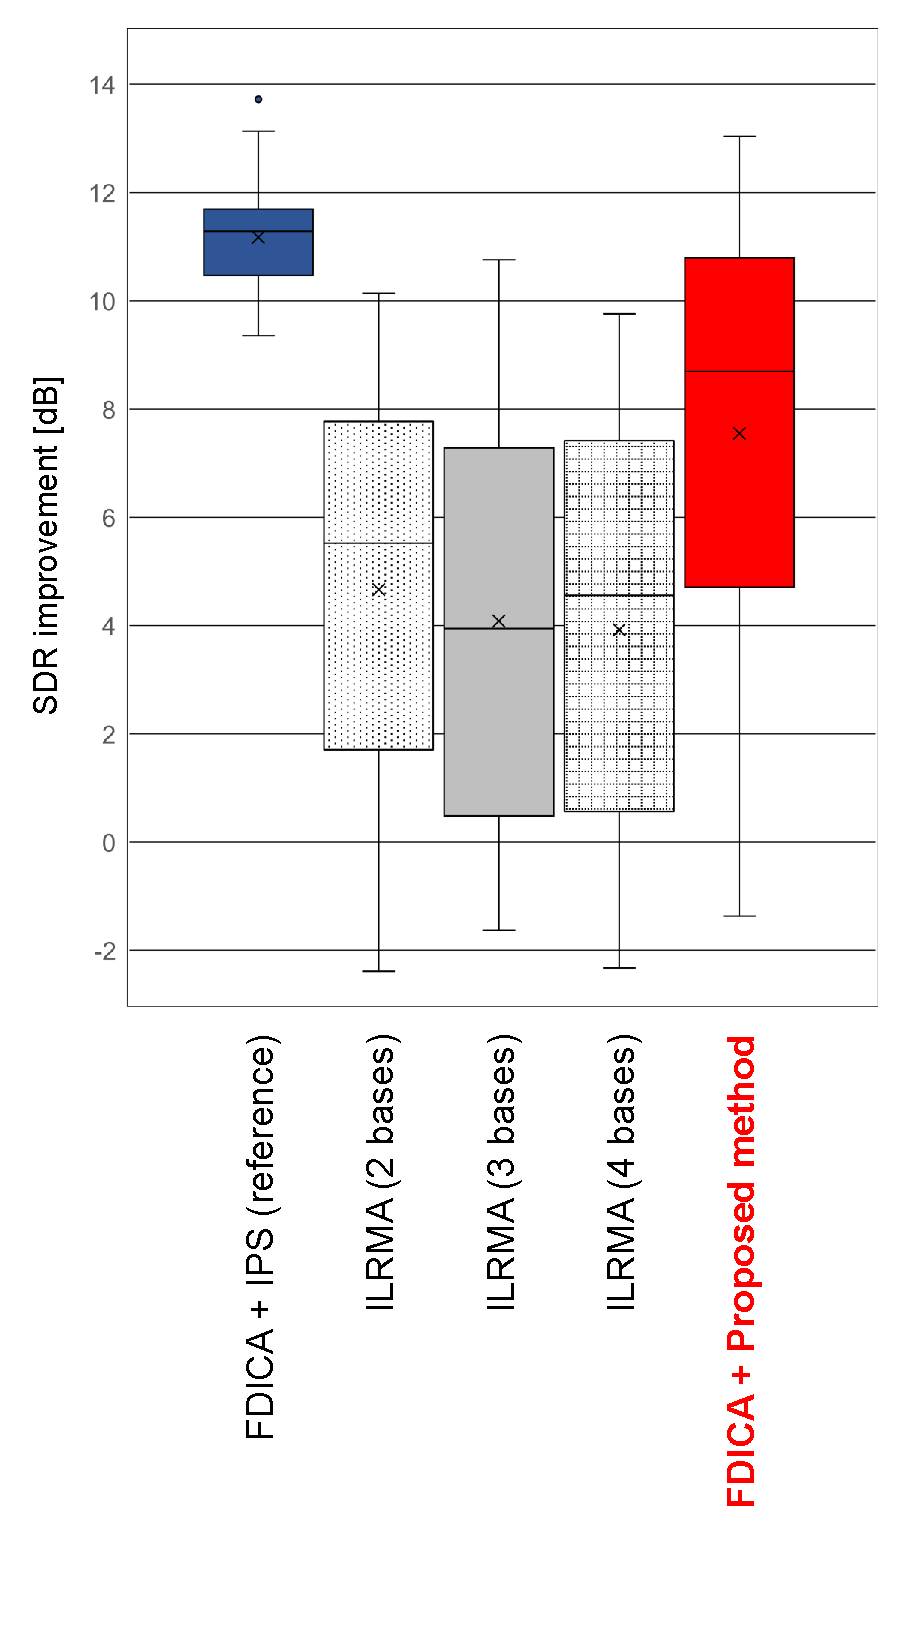
\includegraphics[width=0.7\columnwidth]{figures/sdr_glaph_060-120.eps}
    \end{center}
    \vspace{-8pt}
	\caption{SDR improvements of source directions\\
	\protect\linebreak~($\theta_1$, $\theta_2$)~=~($60^\circ$, $120^\circ$).}
	\label{fig:060-120}
\end{figure}
%%%%%%%%%%%%%%%%%%%%%%%%%%%%
%%%%%%%%%%%%%%%%%%%%%%%%%%%%
\begin{figure}[th]
    \vspace{4pt}
    \begin{center}
        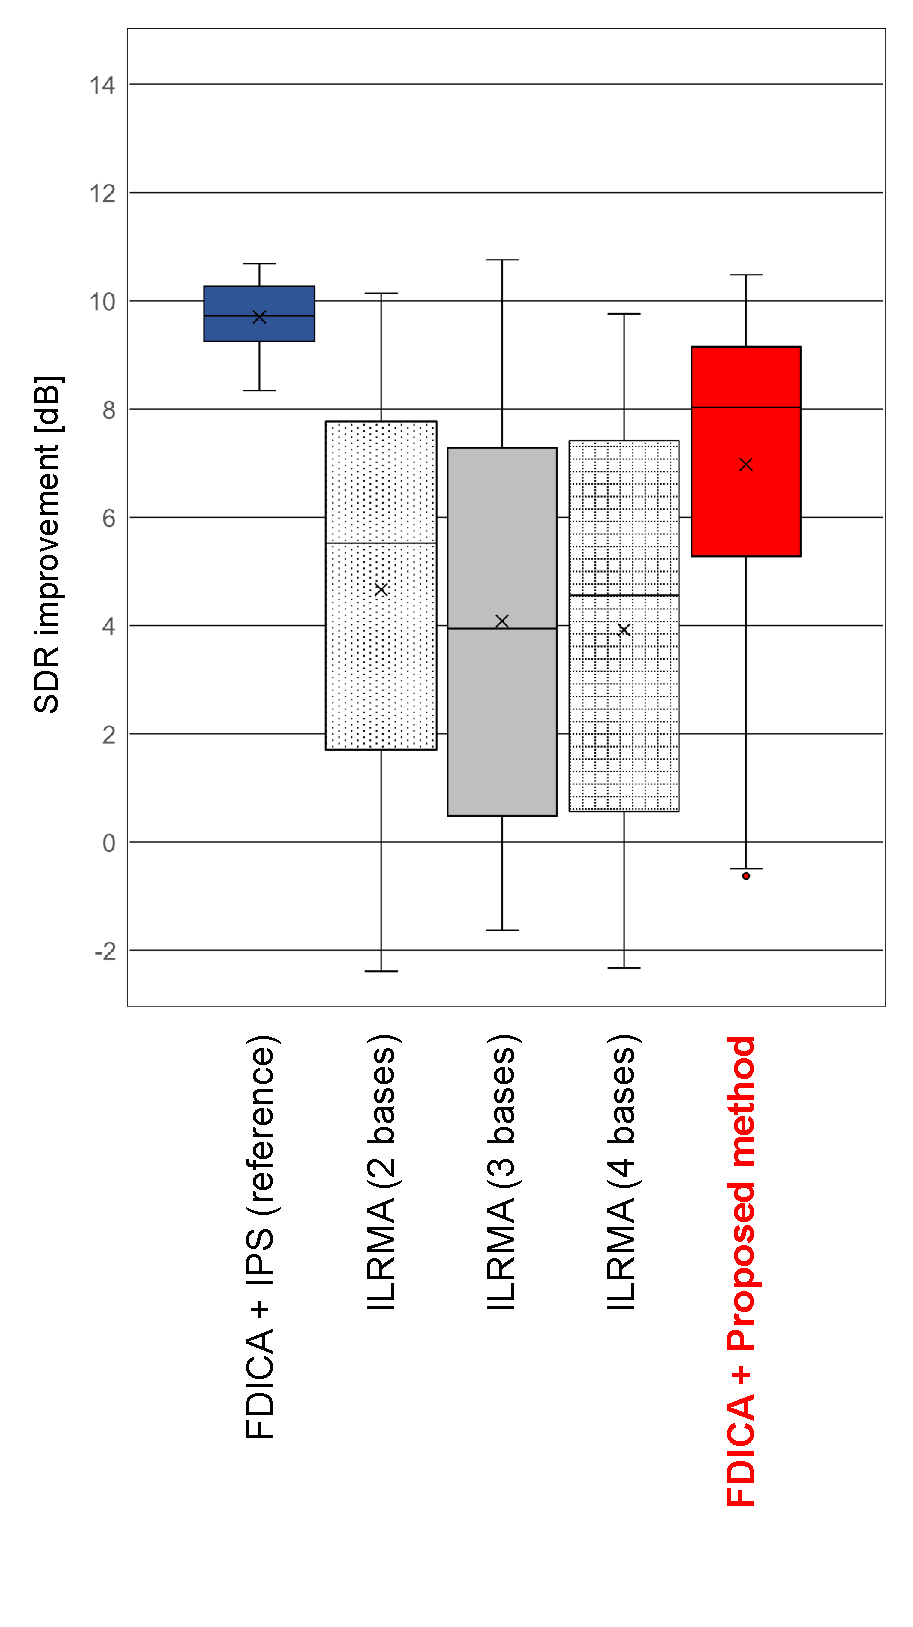
\includegraphics[width=0.7\columnwidth]{figures/sdr_glaph_060-100.eps}
    \end{center}
    \vspace{-8pt}
	\caption{SDR improvements of source directions\\
	\protect\linebreak~($\theta_1$, $\theta_2$)~=~($60^\circ$, $100^\circ$).}
	\label{fig:060-100}
\end{figure}
%%%%%%%%%%%%%%%%%%%%%%%%%%%%
%%%%%%%%%%%%%%%%%%%%%%%%%%%%
\begin{figure}[th]
    \vspace{4pt}
    \begin{center}
        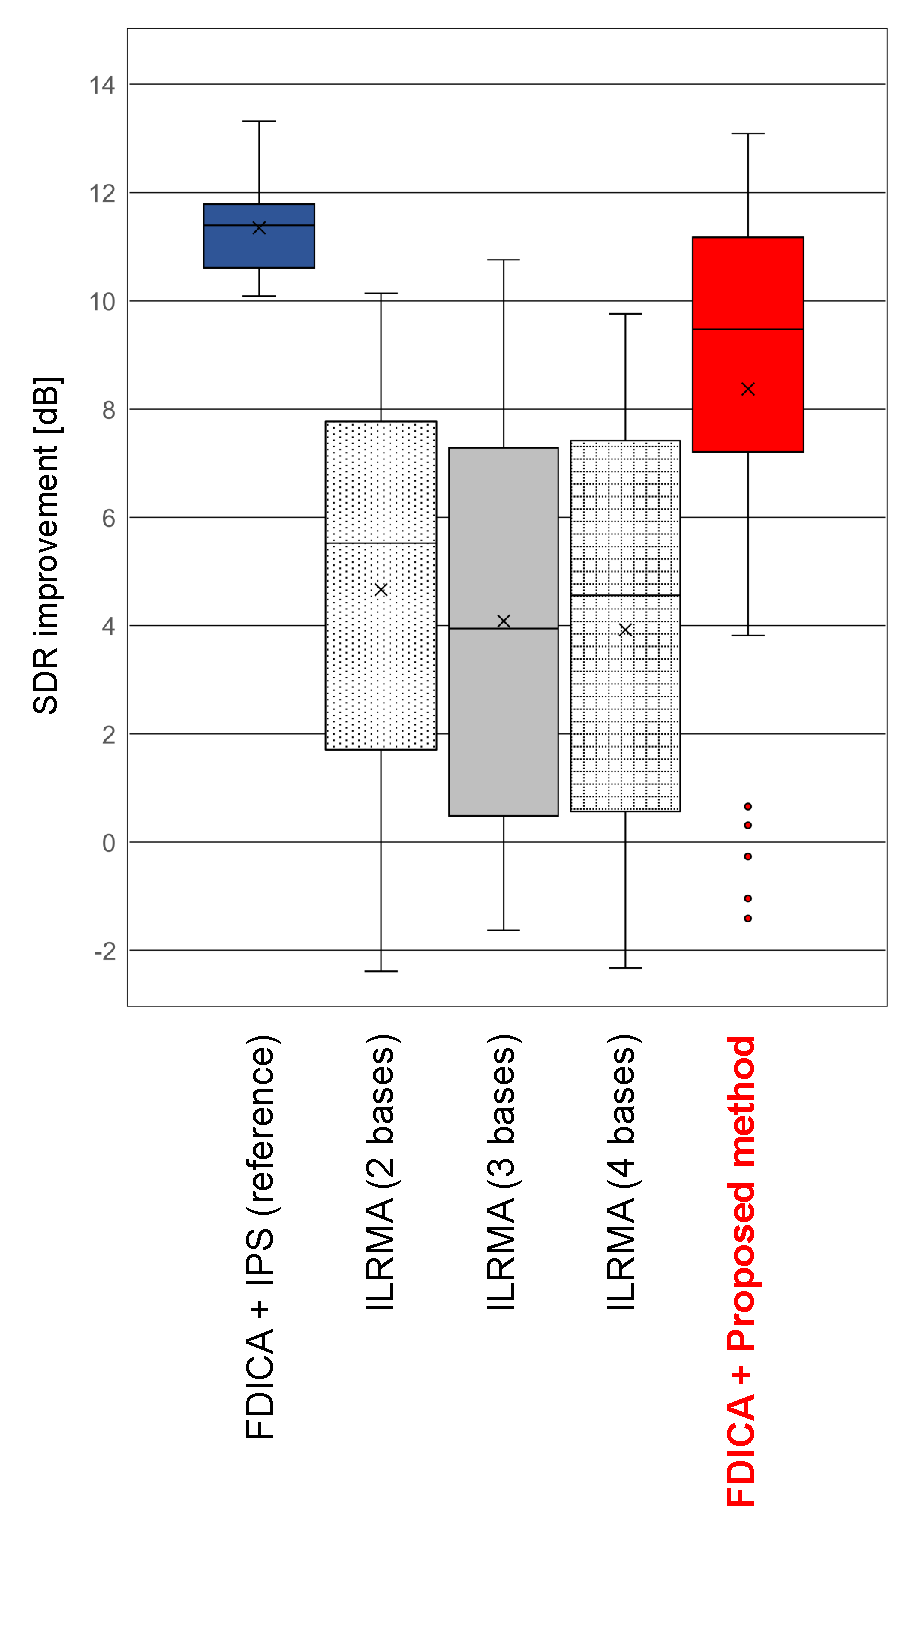
\includegraphics[width=0.7\columnwidth]{figures/sdr_glaph_070-110.eps}
    \end{center}
    \vspace{-8pt}
	\caption{SDR improvements of source directions~($\theta_1$, $\theta_2$)~=~($70^\circ$, $110^\circ$).}
	\label{fig:070-110}
\end{figure}
%%%%%%%%%%%%%%%%%%%%%%%%%%%%
%%%%%%%%%%%%%%%%%%%%%%%%%%%%
\begin{figure}[th]
    \vspace{4pt}
    \begin{center}
        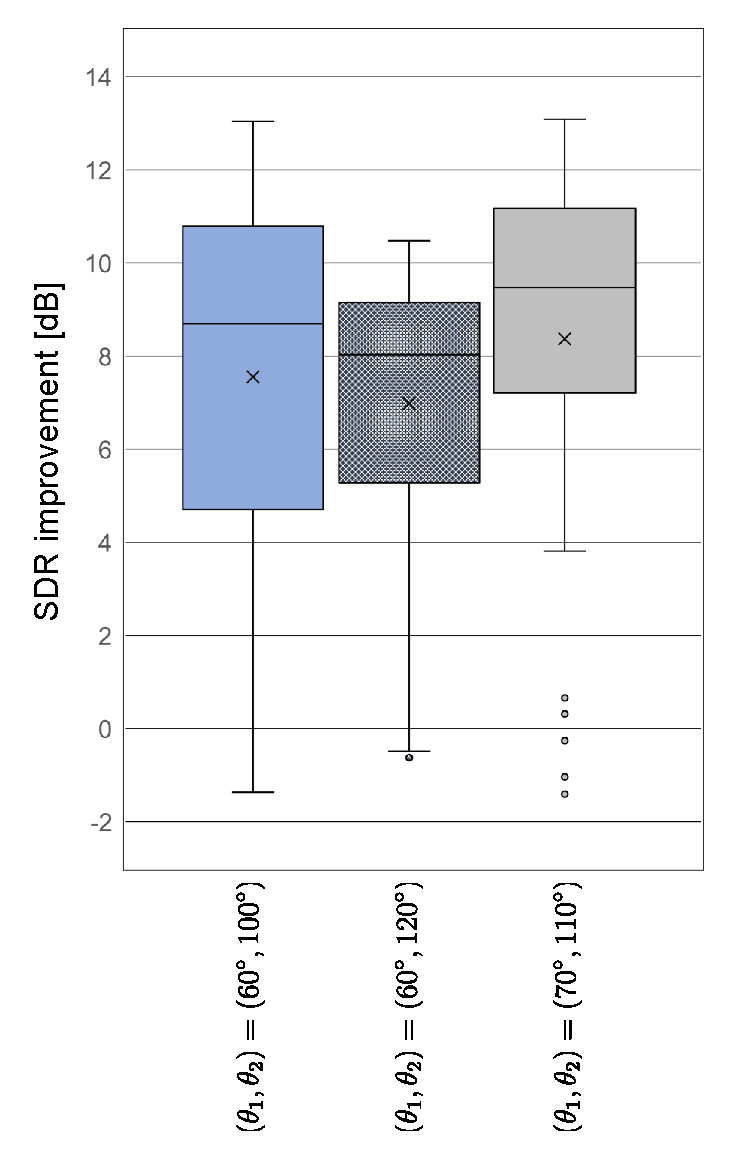
\includegraphics[width=0.7\columnwidth]{figures/sdr_glaph_DOA.eps}
    \end{center}
    \vspace{-8pt}
	\caption{SDR improvement of the proposed method for each direction.}
	\label{fig:DOA}
\end{figure}
%%%%%%%%%%%%%%%%%%%%%%%%%%%%



\clearpage
%----------------------------------------------
\section{本章のまとめ}
\label{sec:matome}
%----------------------------------------------
本章では,提案手法の有効性を確認するため,高残響の音声混合信号に対して音源分離実験を行い,他手法と比較した.
実験の結果,提案手法を適用したFDICAのスコアが平均的にILRMAを上回る結果となった.
また,提案手法は音源の到来方向に依存しないことから,FDICAの一般的なポスト処理として適用可能であることを示した.
次章では,本論文における総括とした結論を述べる.
